\chapter{Semantic SLAM}

\section{DeLS-3D: Deep Localization and Segmentation with a 2D Semantic Map\cite{WangWang2018DeLS}}

\subsection{Abstract}

Sensor fusion scheme: Integrates camera videos, Motion sensors (GPS/IMU), and a 3D semantic map.

步骤:
\begin{itemize}
\item Initial Coarse camera pose obtained from consumer-grade GPS/IMU
\item A label map can be rendered from the 3D semantic map.
\item Rendered label map and the RGB image are jointly fed into a pose CNN, yielding a corrected camera pose.
\item A multi-layer RNN is further deployed improve the pose accuracy
\item Based on pose from RNN, a new label map is rendered
\item New label map and the RGB image is fed into a segment CNN which produces per-pixel sematnic label.
\end{itemize}

从结果可以看出,Scene Parsing以及姿态估计两者可以相互改善,从而提高系统的鲁棒性以及精确度。

\subsection{Introduction}

在Localization中,传统的做法是基于特征匹配来做,但这样的坏处是,如果纹理信息较少,那么系统就不稳定,会出错。一种改进办法是利用深度神经网络提取特征。实际道路中包含大量的相似场景以及重复结构,所以前者实用性较差。

在Scene Parsing中,深度神经网络用的很多,最好的基于(FCN + ResNet)的途径。在视频中,可以借助光流信息来提高计算速度以及时间连续性。对于静态场景,可以借助SfM技术来联合Parse以及Reconstruction.但这些方法十分耗时。

相机的姿态信息可以帮助3D语义地图与2D标签地图之间的像素对应。反过来,场景语义又会帮助姿态估计。

\subsection{Framework}

总的工作流程,如图\ref{DeLSFramework}所示:
\begin{figure}
\centering
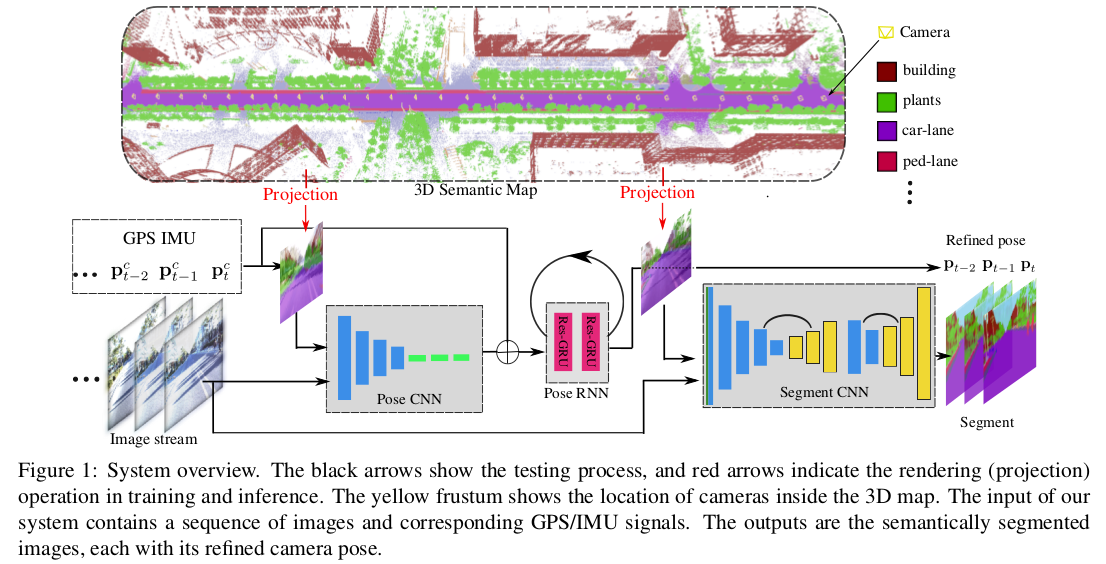
\includegraphics[width=0.95\textwidth]{SemanticSLAM/DeLS1.png}
\caption{DeLS Framwork}
\label{DeLSFramework}
\end{figure}

从图中可以看出,RGB Images 以及 根据GPS/IMU获得的semantic label map被输入到Pose CNN,然后输出的Pose信息输入到Pose RNN来对Pose进一步提高,{\bfseries 这里用RNN来获得前后帧的一致性}!然后在利用新得到的Pose来获取更精确的Semantic Label Map,最后,这个label Map以及RGB图像输入到Segment CNN来进一步提高语义地图的精度。这里标签地图被用于提高语义地图的空间精度以及时间一致性。

网络的训练是基于非常精确地相机姿态以及语义分割,所以可以采用监督学习。

\subsection{Related Work}

\begin{itemize}
\item Camera Pose Estimation

\begin{itemize}
\item PnP

在大的范围内,可能需要提供姿态的先验信息。但对于城市环境中存在大量的Points,这种方法不适用,且不适用于纹理少、结构重复、以及重叠的区域。

\item Deep learned features

PoseNet, LSTM-PoseNet, Bi-Directional LSTM, or Kalman filter LSTM.但实际中由于存在植被等重复性的场景,所以十分有必要加入GPS/IMU等信息来获得鲁棒的定位结果。而在这里,我们采用结合RGB图像与Online Rendered label map的方式来提供更好的结果。

{\bfseries \color{red} 这里问题来了,首先是label map的精度如何?其次,随着时间的变化,label map与实际RGB图像可能完全不同,如季节改变了,这应该如何?}

\end{itemize}

\item Scene Parsing

FCN, Multi-scale context module with dilated convolution, Pooling, CRF, or Spatial RNN with hundreds of layers.这些方法都太耗时了。

一些方法是利用小模型或者模型压缩来加速,但会降低精度。

当输入是Video时,需要考虑时空信息。当前,存在利用光流来帮助label以及semantic在相邻帧之间的传递。借助3D信息以及相机姿态把相邻帧联系起来,可以更好的处理静态背景下的表示。具体的,是使用DeMoN来提高推理效率。

\item Joint 2D-3D for video parsing

CNN-SLAM把传统的3D重建模块替换为深度预测网络,且借助语义分割网络来获取场景语义。同样比较耗时、仅适合静态背景,重建效果也不好。

\end{itemize}

\subsection{Dataset}

\begin{itemize}
\item Data collection

Mobile LIDAR to collect point clouds of the static 3D map. Cameras' resolution: 2018 * 2432.

\item 2D and 3D Labeling

\begin{itemize}
\item Over-segment the point clouds into point clusters based on spatial distances and normal directions, then label each point cluster manually.

\item Prune out the points of static background, label the remaining points of the objects.

\item After 3D-2D projection, only moving object remain unlabeled.

\end{itemize}

\item 使用图形学中的 \textit{Splatting techniques} 来优化未被标签的像素。

\end{itemize}

\subsection{Localizing camera and Scene Parsing}

\subsubsection{Render a label map from a camera pose}

初始的相机的姿态来自于GPS/IMU等传感器。

6-DOF相机姿态:$\mathbf{b} = [\mathbf{q}, \mathbf{t}] \in SE(3)$. 其中$\mathbf{q} \in SO(3)$是四元数表示的旋转,$\mathbf{t} \in \mathbb{R}^3$表示Translation。

在由Point经Spaltting获取其面时,面积大小$s_c$根据Point所属的类别来决定,且与该类别与相机的平均距离的比例有关。

\begin{displaymath}
s_c \propto \frac{1}{|\mathcal{P}_c|}\sum_{x \in \mathcal{P}_c}\min_{\mathbf{t}\in \tau}d(x, t)
\end{displaymath}

其中,$P_c$是属于类别$c$的3D点云,$\tau$是精确地相机姿态。如果面积过大,则会出现Dilated edges,而如果面积过小,则会形成Holes。

\subsubsection{Camera Localization rectification with road prior}

\textbf{CNN-GRU pose Network Architecture}

文中的Pose Network包含一个Pose CNN以及一个Pose GRU-RNN。其中Pose CNN的输入是RGB图像I以及一个标签地图L。输出是一个7维的向量,表示输入图像I与输入标签地图L(由较粗糙的姿态$\mathbf{p}_i^c$得到)之间的位姿关系,从而得到一个在3D Map中更精确的姿态:
$\mathbf{P}_i = \mathbf{p}_i^c + \hat{\mathbf{p}}_i$。

CNN结构借鉴DeMoN,利用打的Kernel Size来获取更大的内容,同时保证运行效率,减少参数量。

由于输入的是图像流,为了保证时间一致性,所以在Pose CNN之后又加上一个多层的GRU网络,且该网络具有Residual Connection的连接结构。结果表明,RNN相比于卡尔曼滤波可以获得更好的运动估计。

\textbf{Pose Loss}

类似于PoseNet的选择,使用Geometric Matching Loss来训练。

\subsubsection{Video Parsing with Pose Guidance}

上一步得到的Pose估计,不是完美的,因为存在light poles存在。由于反光,很多点消失了。此外,由于存在动态物体,这些物体可能在原来的标签地图中不存在,所以这些区域可能发生错误。因此,利用额外的一个Segment CNN来出来这些问题。且利用标签地图来指导分割过程。

\textbf{Segment Network Architecture}

首先基于RGB图像对该网络训练,然后加入标签地图数据进行微调(Fine Tune).具体结构如图\ref{SegmentDeLS}所示。

\begin{figure}[!hbtp]
\centering
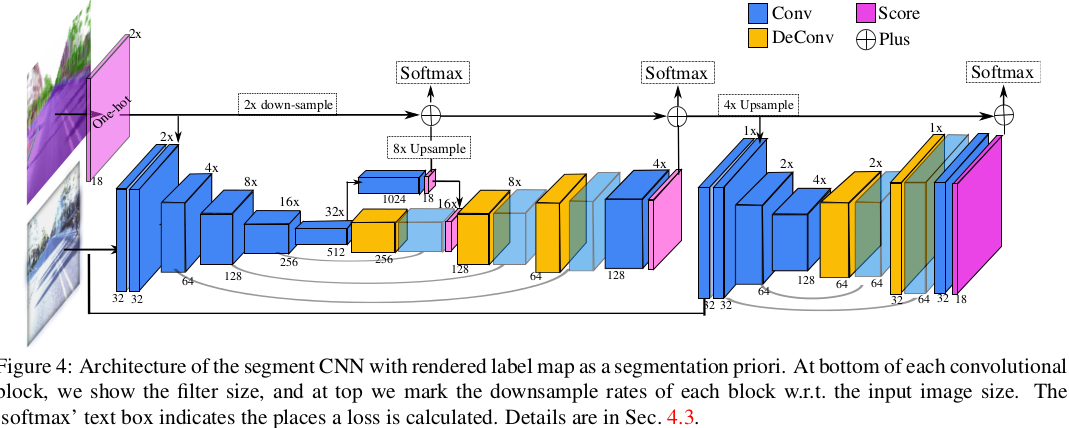
\includegraphics[width=0.95\textwidth]{SemanticSLAM/DeLS2.png}
\caption{Segment Network in DeLS}
\label{SegmentDeLS}
\end{figure}

需要注意的是,当标签地图加入框架时,需要经过编码,即每一个像素经One-hot操作得到一个32维的Feature Representation。然后得到的32维特征加入到RGB图像的第一层卷积输出中,且该层的Kernel数也是32个,从而平衡了两种数据的通道数(Channel Number)。

\subsection{Experiment}

\begin{itemize}
\item Adopt OpenGL to efficiently render a label map with the z-buffer handling. 

\item Implement all the networks by adopting the MXNet platform.

\item 使用RNN可以提高Pose的精度,也可以提高Segment的精度,尤其对于纤细的物体。

\end{itemize}

\subsection{Conclusion}

基于已有的3D语义地图以及视频数据,实现相机的姿态、场景语义任务的实现。算法融合了多种传感器信息。实验表明,相机位姿估计与场景语义两类任务可以相互促进、提高。

\section{PAD-Net: Multi-Task Guided Prediction-and-Distillation Network for Simultaneous Depth and Scene Parsing \cite{Xu2018PADNet}}

\subsection{Abstract}

利用同一个网络,完成深度估计与场景解析两个任务。具体来说,通过神经网络学习一系列的中间辅助任务(Intermediate Auxiliary Tasks),然后基于中间任务的输出,作为多模式数据(Multi-modal  input)输入到下一层网络中,完成最终的深度估计以及场景解析两个任务。

其中,一系列的中间任务包括低层任务和高层任务。低层任务包括:Surface Normal, Contour;高层任务包括:Depth Estimation, Scene Parsing.

\subsection{Analysis}

\subsubsection{Effect of Direct Multi-task Learning}
It can be observed that on NYUD-v2, the Front-end + DE + SP slightly outperforms the Front-end
+ DE, while on Cityscapes, the performance of Front-end + DE + SP is even decreased, which means that using a direct multi-task learning as traditional is probably not an effective means to facilitate each other the performance of different tasks. (DE: Depth Estimation, SP: Scene Parsing)

\subsubsection{Effect of Multi-modal Distillation}
这种Multi-Modal Distillation对结果十分有效。且:
\begin{quote}
By using the attention PAD-Net (Distillation C + SP) guided scheme, the performance of the module C is further improved over the module B.
\end{quote}

\subsubsection{Importance of Intermediate Supervision and Tasks}

测试了选择不同的中间任务类型,如:(Multi-Task Deep Network)MTDN + inp2(depth + semantic map), MTDN+3inp3(depth + semantic + surface normal), MTDN + all(depth + semantic + surface + contour).

其中MTDN + all比MTDN + 0-3都好。

\section{RNN for Learning Dense Depth and Ego-Motion from Video}









